\documentclass[11pt, a4paper]{article}
\usepackage[T1]{fontenc}
\usepackage[utf8]{inputenc}
\usepackage[MeX]{polski}
\usepackage[polish]{babel}
\usepackage{enumerate}
\usepackage{float}
\usepackage{geometry}
\usepackage{amsmath}
\usepackage[linesnumbered,ruled]{algorithm2e}
\usepackage{graphicx}
\usepackage{caption}

\SetKw{KwDownTo}{downto}
\graphicspath{{../plots/}}

\geometry{top=1.5cm, bottom=1.5cm, right=1.5cm, left=1.5cm}


\title{Obliczenia naukowe\\Lista4}
\author{Stanisław Woźniak}
\date{}

\begin{document}
    \maketitle
    \section{Zadanie 1.}
    \subsection{Ilorazy różnicowe}
    \subsection{Opis}
    \subsection{Pseudokod}
    \section{Zadanie 2.}
    \subsection{Wielomian interpolacyjny Newtona}
    \subsection{Opis}
    Wielomian interpolacyjny Newtona jest to wielomian, który interpoluje podaną funkcję $f$ oraz jest postaci podanej poniżej.\\
    \centerline{\textbf{Postać Newtona wielomianu}}
    $$ N_{n}(x) = f[x_{0}] + f[x_{0}, x_{1}](x - x_{0}) + ... + f[x_{0}, x_{1}, x_{2},...,x_{n}](x - x_{0})(x - x_{1})...(x - x_{n-1})$$
    $$ N_{n}(x) = f[x_{0}] + \sum_{k=1}^{n} (f[x_{0},.., x_{k}]\prod_{j=0}^{k-1} (x - x_{j}))$$

    Zadanie polegało na zaimplementowaniu funkcji, która z pomocą algorytmu Hornera wylicza wartość wielomianu postaci Newtona.\\
    \centerline{\textbf{Uogólniony algorytm Hornera}}
    $$ w_{n}(x) = f[x_{0},...,x_{n}]$$
    $$ w_{i}(x) = f[x_{0},...,x_{i}] + (x - x_{i})w_{i+1}(x)$$
    $$i = n-1,...,0$$
    \centerline{\textbf{Związek pomiędzy wartością wielomianu Newtona a algorytmem Hornera}}
    $$ N_{n}(x) = w_{0}(x)$$


    \subsection{Pseudokod}
    \begin{algorithm}[H]
        \SetKwInOut{Input}{Input}
        \SetKwInOut{Output}{Output}

        \underline{warNewton} $(x , fx,t)$\;
        \Input{x - wektor węzłów, fx - wektor wartości odpowiednich węzłów z wektora x, t - argument wielomianu}
        \Output{nt}
        $n \gets length(x)$; $nt \gets fx[n]$\;
        \For{$i \gets n-1$ \KwDownTo $1$}{
            $nt \gets  fx[i] + (t - x[i])*nt$\;
        }
        return $nt$\;
        \caption{Wyliczenie wartości wielomianu Newtona używając uogólnionego algorytmu Hornera}
    \end{algorithm}
    \section{Zadanie 3.}
    \subsection{Postać naturalna wielomianu interpolacyjnego Newtona}
    \subsection{Opis}
    \subsection{Pseudokod}
    \section{Zadanie 4.}
    \subsection{Rysowanie wykresów}
    \subsection{Opis}
    \subsection{Pseudokod}
    \section{Zadanie 5.}
    \subsection{Problem}
    W zadaniu został przedstawiony problem polegający na porównaniu dwóch funkcji z ich wielomianami interpolacyjnymi stopnia n używając powyższych funkcji oraz podanych przedziałów rysowania.\\
    \\
    $n \in \{5, 10, 15\}$\\
    $a(x) = e^{x}$, przedział rysowania: $[0,1]$\\
    $b(x) = x^2\sin{x}$, przedział rysowania: $[-1, 1]$
    \subsection{Wyniki}
    Objaśnienie wykresów:\\
    y1 (kolor niebieski) - graficzne przedstawienie wyliczonyego wielomianu interpolacyjnego.\\
    y2 (kolor czerwony) - graficzne przedstawienie podanej funkcji.
    \begin{figure}[H]
        \captionsetup{labelformat = empty}
        \begin{minipage}{0.5\textwidth}
            \centerline{\textbf{Wykresy funkcji a:}}
            \caption{$n=5$}
            \centering
            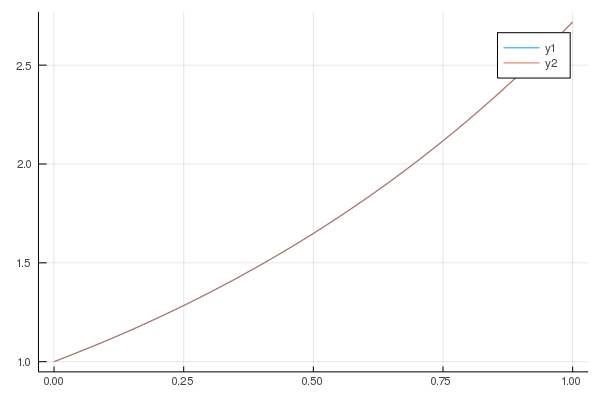
\includegraphics[width=\linewidth]{plot-5_a_n5}
        \end{minipage}
        \begin{minipage}{0.5\textwidth}
            \centerline{\textbf{Wykresy Funkcji b:}}
            \caption{$n=5$}
            \centering
            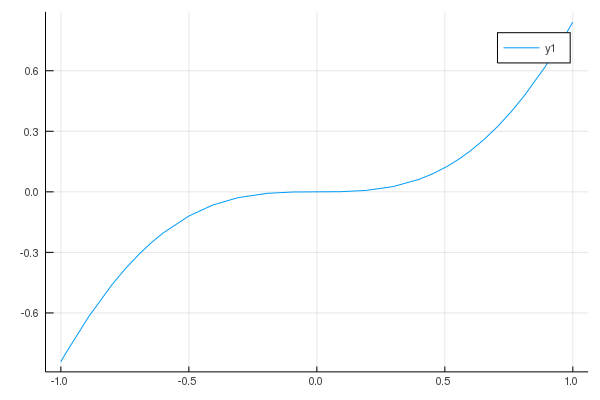
\includegraphics[width=\linewidth]{plot-5_b_n5}
        \end{minipage}

        \begin{minipage}{0.5\textwidth}
            \caption{$n=10$}
            \centering
            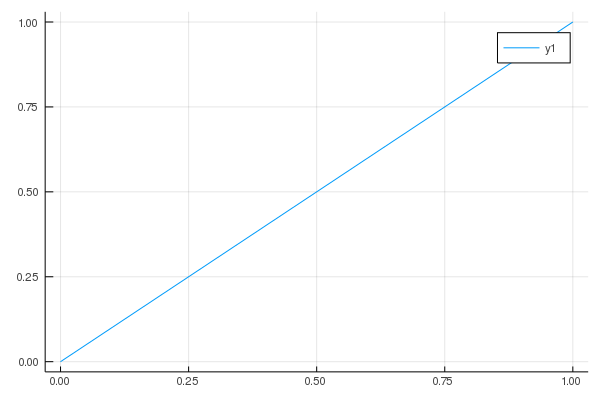
\includegraphics[width=\linewidth]{plot-5_a_n10}
        \end{minipage}
        \begin{minipage}{0.5\textwidth}
            \caption{$n=10$}
            \centering
            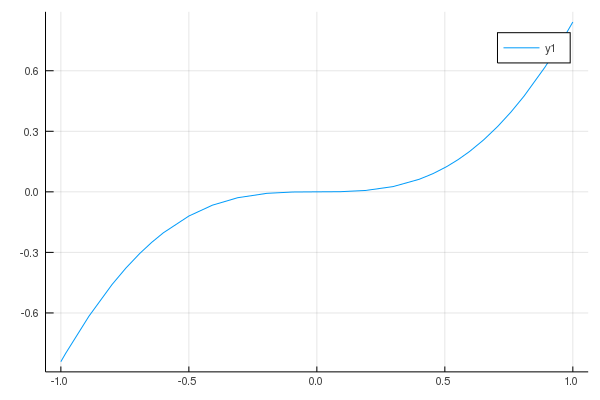
\includegraphics[width=\linewidth]{plot-5_b_n10}
        \end{minipage}
        
        \begin{minipage}{0.5\textwidth}
            \caption{$n=15$}
            \centering
            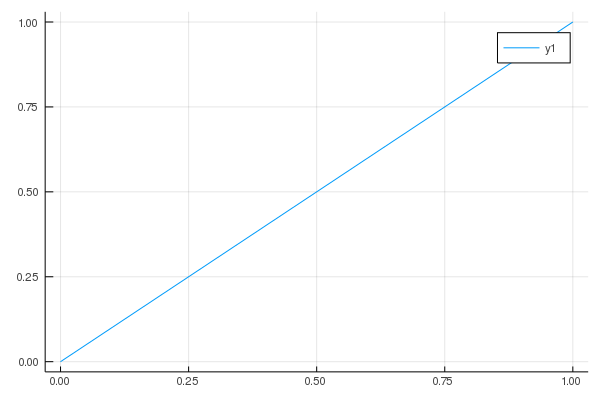
\includegraphics[width=\linewidth]{plot-5_a_n15}
        \end{minipage}
        \begin{minipage}{0.5\textwidth}
            \caption{$n=15$}
            \centering
            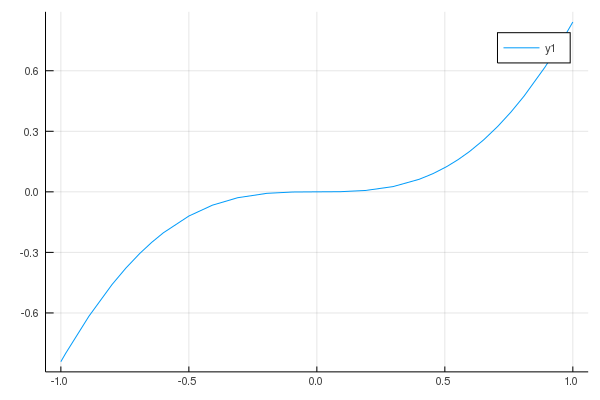
\includegraphics[width=\linewidth]{plot-5_b_n15}
        \end{minipage}
    \end{figure}
    \subsection{Wnioski}


    TODO



    \section{Zadanie 6.}
    \subsection{Problem}
    Problemem w zadaniu było pokazanie na wykresach podane funkcjie oraz ich wielomiany interpolacyjne stopnia n.\\
    \\
    $n \in \{5, 10, 15\}$\\
    $a(x) = |x|$, przedział rysowania: $[-1,1]$\\
    $b(x) = \frac{1}{1 + x^2}$, przedział rysowania: $[-5, 5]$
    \subsection{Wyniki}
    Objaśnienie wykresów:\\
    y1 (kolor niebieski) - graficzne przedstawienie wyliczonyego wielomianu interpolacyjnego.\\
    y2 (kolor czerwony) - graficzne przedstawienie podanej funkcji.
    \begin{figure}[H]
        \captionsetup{labelformat = empty}
        \begin{minipage}{0.5\textwidth}
            \centerline{\textbf{Wykresy funkcji a:}}
            \caption{$n=5$}
            \centering
            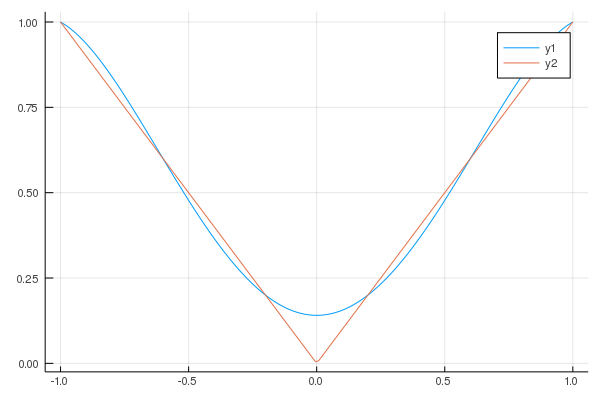
\includegraphics[width=\linewidth]{plot-6_a_n5}
        \end{minipage}
        \begin{minipage}{0.5\textwidth}
            \centerline{\textbf{Wykresy Funkcji b:}}
            \caption{$n=5$}
            \centering
            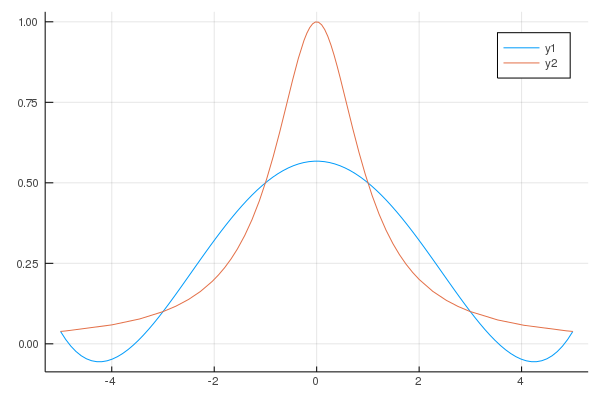
\includegraphics[width=\linewidth]{plot-6_b_n5}
        \end{minipage}

        \begin{minipage}{0.5\textwidth}
            \caption{$n=10$}
            \centering
            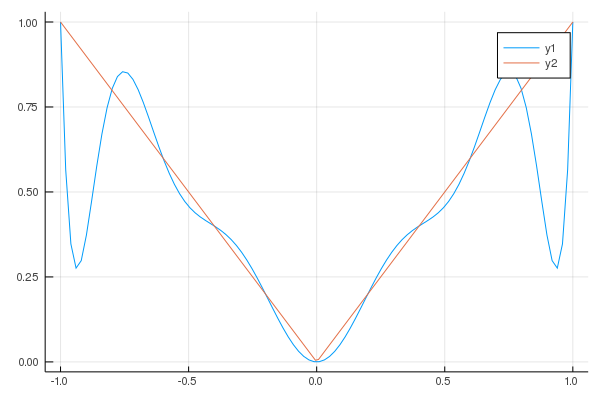
\includegraphics[width=\linewidth]{plot-6_a_n10}
        \end{minipage}
        \begin{minipage}{0.5\textwidth}
            \caption{$n=10$}
            \centering
            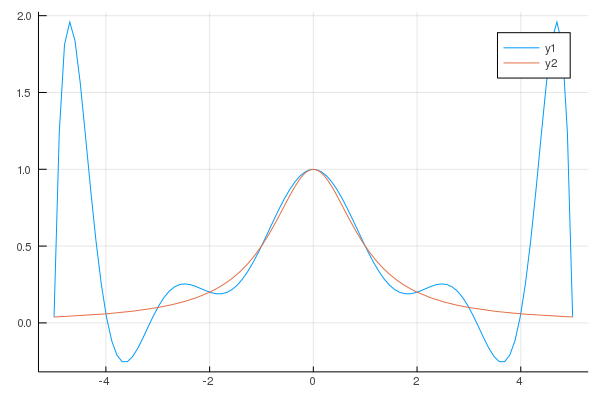
\includegraphics[width=\linewidth]{plot-6_b_n10}
        \end{minipage}
        
        \begin{minipage}{0.5\textwidth}
            \caption{$n=15$}
            \centering
            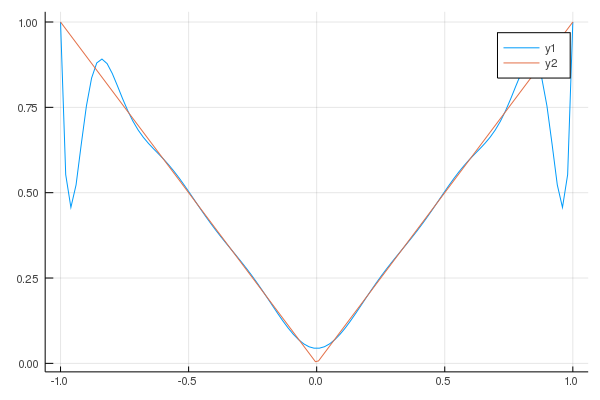
\includegraphics[width=\linewidth]{plot-6_a_n15}
        \end{minipage}
        \begin{minipage}{0.5\textwidth}
            \caption{$n=15$}
            \centering
            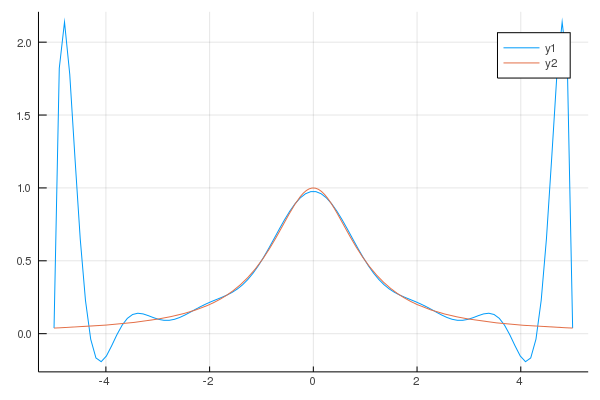
\includegraphics[width=\linewidth]{plot-6_b_n15}
        \end{minipage}
    \end{figure}
    \subsection{Wnioski}


    TODO

\end{document}